%===============================================================
% CHAPTER 6 – Structural and Aerodynamic Simulation (FEA & CFD)
%===============================================================
\chapter{Structural and Aerodynamic Simulation (FEA \& CFD)}
\label{ch:simulation}

To rigorously validate the structural integrity and aerodynamic efficiency of the Solift UAV during critical flight phases, comprehensive simulation analyses were conducted. This chapter details the Finite Element Analysis (FEA) performed on the primary wing structure using SolidWorks Simulation, followed by a Computational Fluid Dynamics (CFD) evaluation of the full aircraft configuration in cruise mode using ANSYS Fluent.

\section{Static Stress Analysis of the Main Wing Structure}
\label{sec:static_stress}

A linear static stress analysis was executed to evaluate the structural response of the main wing under anticipated aerodynamic loading. Within the simulation environment, the wing root was assigned a fixed geometry constraint, simulating a rigid attachment to the fuselage. A combination of distributed aerodynamic forces and concentrated loads (including a total distributed load of \SI{70}{\newton} and localized vertical loads of \SI{40}{\newton}) were applied to the lifting surfaces to replicate steady-state cruise conditions. 

\begin{figure}[H]
    \centering
    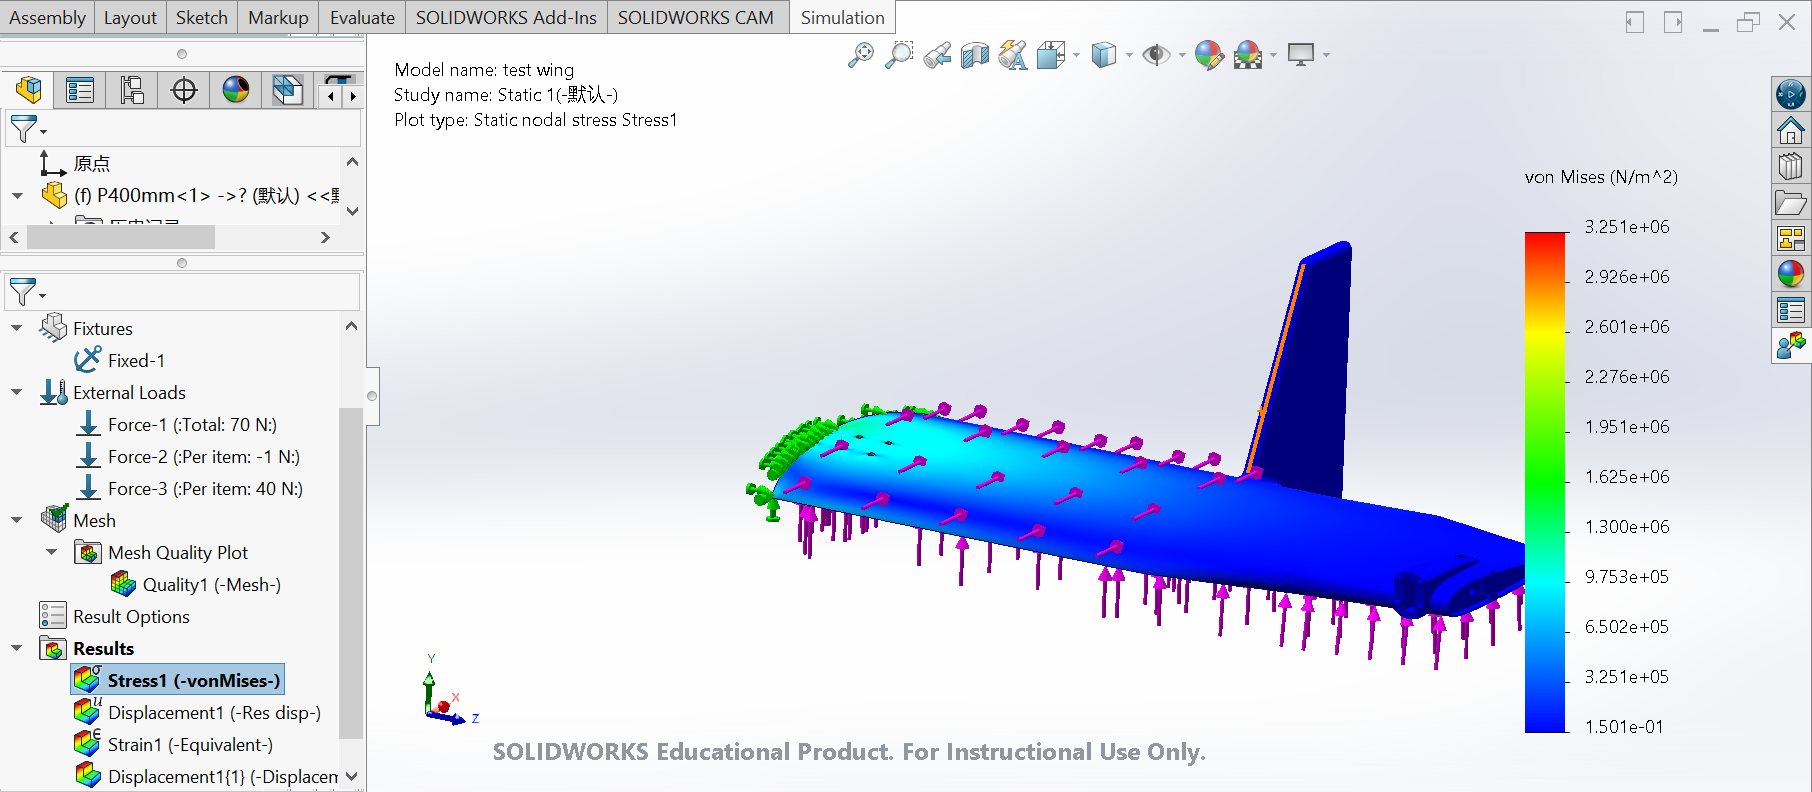
\includegraphics[width=0.9\textwidth]{figures/fea_wing_stress.png}
    \caption{von Mises stress distribution of the main wing under simulated cruise aerodynamic loading (SolidWorks Simulation).}
    \label{fig:fea_stress}
\end{figure}

The resulting von Mises stress distribution (Figure \ref{fig:fea_stress}) indicates a highly uniform load transfer across the wing span. The maximum equivalent stress is localized near the junction of the wing root and the fixed boundary, peaking at approximately \SI{3.251e5}{\newton\per\meter\squared} (\SI{0.325}{\mega\pascal}). This peak stress value is orders of magnitude lower than the typical yield strength of standard aerospace materials, such as carbon fibre composites or aerospace-grade aluminium alloys. The substantial margin of safety confirms that the current wing structural design is highly robust, effectively mitigating any risk of structural failure or material yielding under nominal flight envelopes.

\section{Structural Displacement and Stiffness Evaluation}
\label{sec:displacement}

Under identical boundary conditions and loading scenarios, a displacement analysis was performed to quantify the structural deformation of the wing. 

\begin{figure}[H]
    \centering
    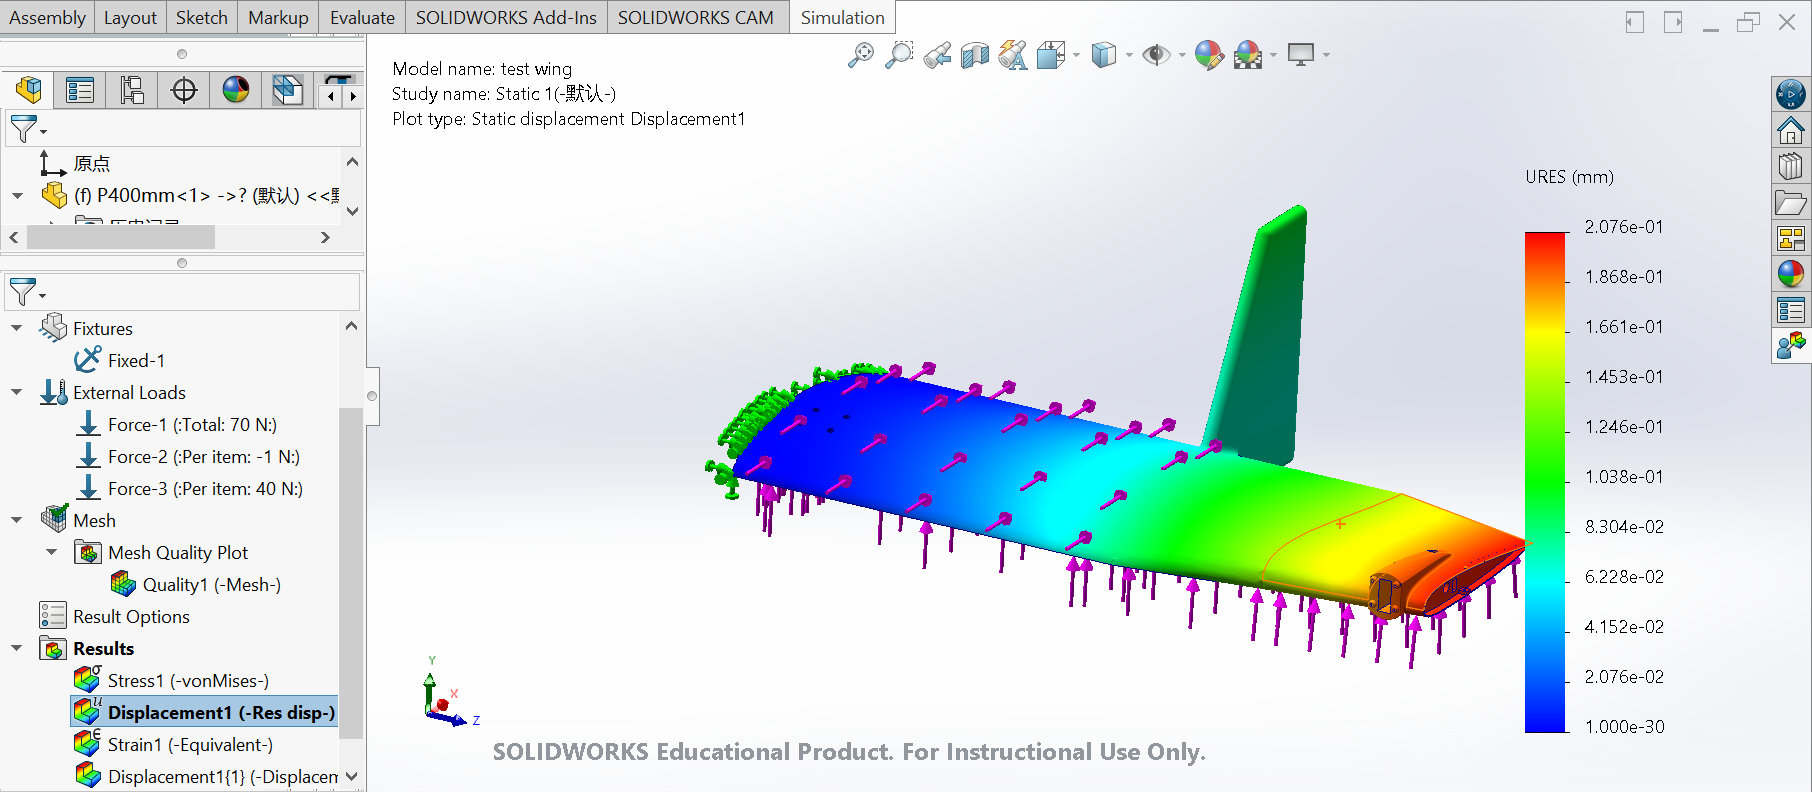
\includegraphics[width=0.9\textwidth]{figures/fea_wing_displacement.png}
    \caption{Resultant displacement (URES) contour map of the main wing structure.}
    \label{fig:fea_displacement}
\end{figure}

The displacement contour map (Figure \ref{fig:fea_displacement}) demonstrates that the maximum resultant displacement (URES) occurs at the wingtip, with a peak deflection of merely \SI{0.207}{\milli\meter}. For a UAV of this scale, a sub-millimetre structural deflection is virtually negligible, indicating exceptional structural stiffness. This high degree of rigidity is critical for the Solift project for two primary reasons: first, it prevents adverse aeroelastic phenomena such as divergence or flutter during high-speed forward flight; second, it ensures that the tilt-rotor mechanisms maintain their precise alignment during transition phases, thereby preserving the intended aerodynamic profile and ensuring flight control accuracy.

\section{Aerodynamic Performance in Cruise Regime (CFD)}
\label{sec:cfd_cruise}

Given the solar-powered nature of the Solift UAV, aerodynamic efficiency directly dictates the energy budget and maximum endurance. To evaluate this, a 3D fluid flow simulation was conducted using ANSYS Fluent to analyze the aerodynamic characteristics of the full vehicle in the forward-flight Cruise Mode.

\begin{figure}[H]
    \centering
    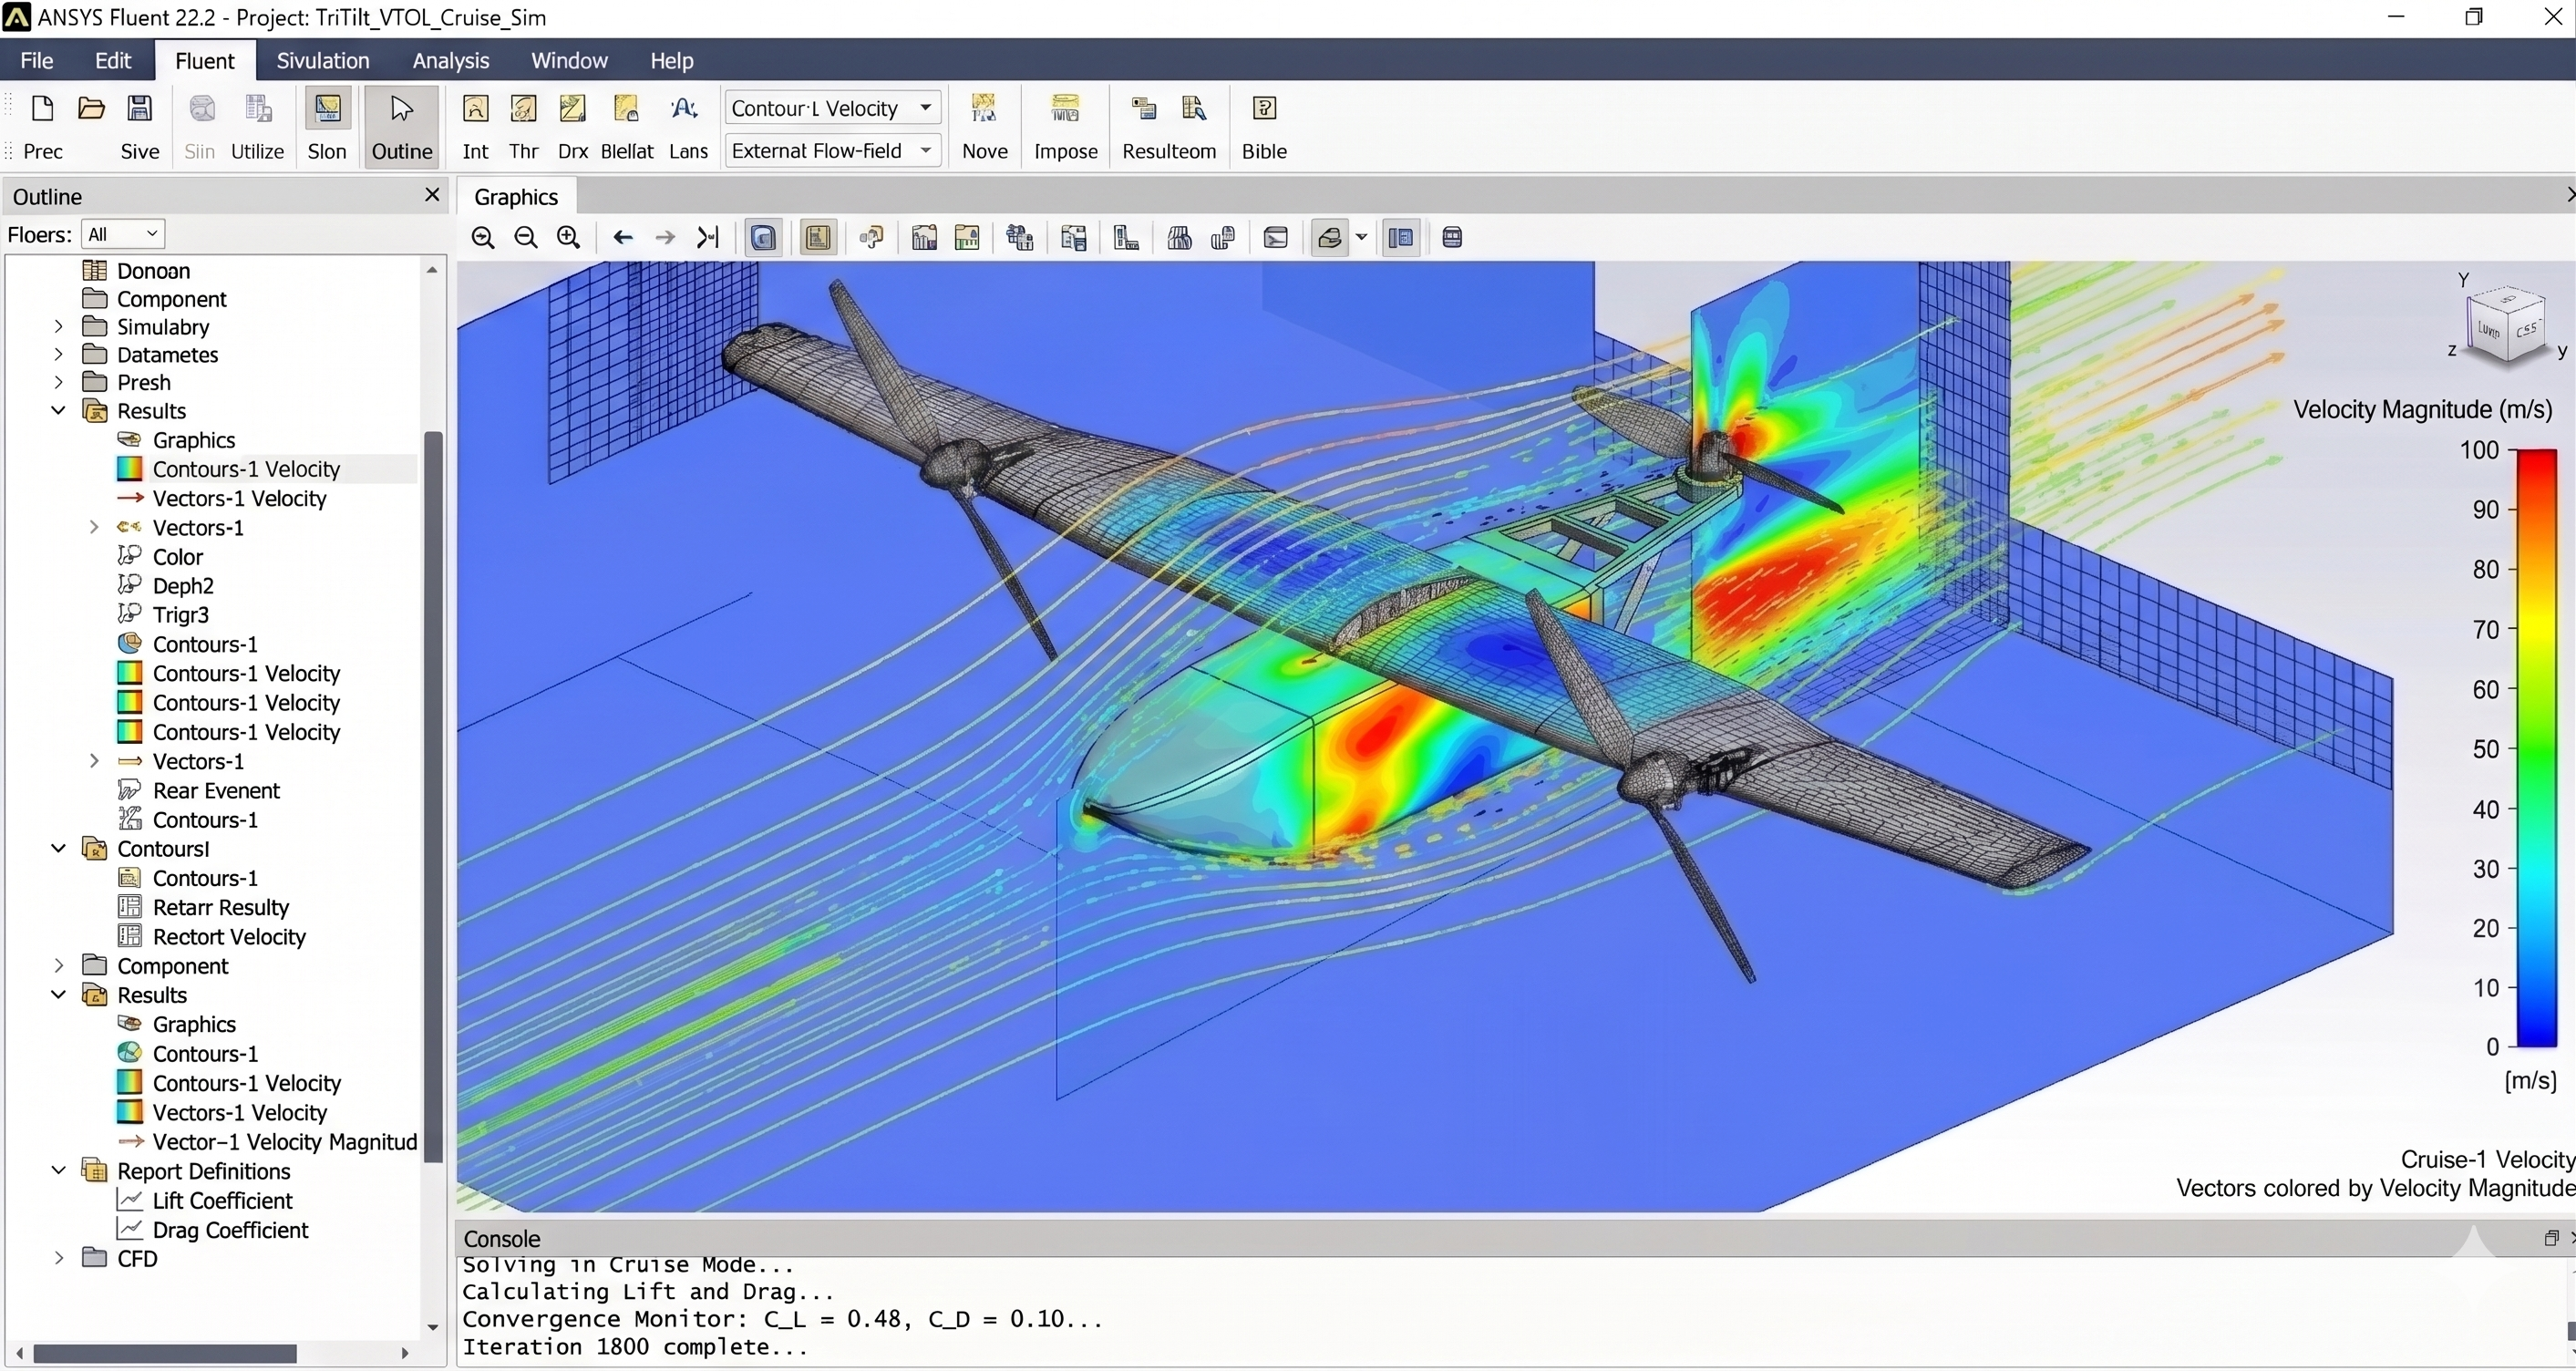
\includegraphics[width=0.95\textwidth]{figures/cfd_cruise_simulation.png}
    \caption{Velocity contours and streamline visualization of the Solift UAV in cruise configuration (ANSYS Fluent).}
    \label{fig:cfd_cruise}
\end{figure}

The velocity contours and streamline visualizations (Figure \ref{fig:cfd_cruise}) confirm excellent boundary layer attachment across the leading edges and the main wing surfaces, with no significant areas of flow separation observed. The wake region behind the fuselage and trailing edges exhibits smooth flow transitions, indicative of a highly streamlined aerodynamic profile. Upon achieving computational convergence (Iteration 1800), the system recorded the following primary aerodynamic coefficients:

\begin{itemize}[noitemsep]
    \item \textbf{Lift Coefficient ($C_L$):} $0.48$
    \item \textbf{Drag Coefficient ($C_D$):} $0.10$
\end{itemize}

These results yield a Lift-to-Drag (L/D) ratio of $4.8$, which represents a highly competitive aerodynamic efficiency for a tilt-rotor platform in this weight class. The smooth integration of the fuselage significantly minimizes form drag, while the main wing generates stable and sufficient lift. This optimized aerodynamic performance is instrumental in minimizing power consumption during cruise, thereby maximizing the operational viability of the solar photovoltaic subsystem and extending the overall flight range.